% !TEX root = ../main.tex

\section{Поняття випадкової величини та її задання}
\begin{definition}
    \emph{Випадковою величиною} називається дійснозначна вимірна функція, що здійснює 
    відображення з $\Omega$ в $\mathbb{R}$, тобто $\xi = \xi(\omega): \Omega 
    \mapsto \mathbb{R}$.
\end{definition}
\begin{remark}
    Вимірність функції $\xi(\omega)$ означає, що 
    \begin{equation}\label{eq:measurable}
        \forall x \in \mathbb{R}: 
        \left\{ \omega \in \Omega\; |\; \xi(\omega) < x\right\} \in \mathcal{F}
    \end{equation} В курсі 
    функціонального аналізу доводиться, що якщо виконується \eqref{eq:measurable}, то
    $\left\{ \omega \; |\; \xi(\omega) > x\right\}$, $\left\{ \omega \; |\; \xi(\omega) \leq x\right\}$,
    $\left\{ \omega \; |\; \xi(\omega) \geq x\right\}$, $\left\{ \omega \; |\; \xi(\omega) = x\right\}$ та
    $\left\{ \omega \; |\; \xi(\omega) \in \left< a; b\right> \right\}$ також належать $\mathcal{F}$.
\end{remark}

В курсі розглядаються випадкові величини двох видів --- дискретні (ДВВ) та неперервні (НВВ).

\subsection{Дискретні випадкові величини та їх задання}
\begin{definition}
    Випадкова величина $\xi = \xi(\omega)$ називається 
    \emph{дискретною випадковою величиною} (ДВВ), якщо вона набуває скінченну або зліченну 
    кількість значень.
\end{definition}
Для задання ДВВ, крім знання значень випадкової величини, необхідно знати ймовірності, 
з якими ці значення приймаються.
$$p_i = P\left\{\omega: \xi(\omega) = x_i\right\} = P(\xi = x_i), i = 1,2,... , \; \sum_{i=1}^\infty p_i = 1$$

\begin{definition}
    \emph{Законом розподілу (ймовірностей)} ДВВ називається співвідношення, яке вказує, 
    які значення ця випадкова величина приймає та з якими ймовірностями.

    Закон розподілу ДВВ записується у вигляді \emph{ряду розподілу}:

    \begin{tabular}{c|c|c|c|c|c}
        $\xi$ & $x_1$ & $x_2$ & ... & $x_n$ & ... \\
        \hline
        $p$ & $p_1$ & $p_2$ & ... & $p_n$ & ...
    \end{tabular}
    \hspace{40pt}
    $x_1 < x_2 < ... < x_n < ...,\; \sum\limits_i p_i = 1$
\end{definition}
\begin{example}
    $\xi$ задає кількість влучень при чотирьох пострілах з імовірністю влучення 
    $p = \frac{1}{2}$. Скласти закон розподілу цієї випадкової величини.

    З формули Бернуллі $P(\xi = k) = C_4^k \left(\frac{1}{2}\right)^k \left(\frac{1}{2}\right)^{4-k} = 
    C_4^k \left(\frac{1}{2}\right)^4 = \frac{C_4^k}{2^4}, k = 0,1,2,3,4$.

    \begin{tabular}{c|c|c|c|c|c}
        $\xi$ & 0 & 1 & 2 & 3 & 4 \\
        \hline
        $p$ & $\frac{1}{2^4}$ & $\frac{4}{2^4}$ & $\frac{6}{2^4}$ & $\frac{5}{2^4}$ & 
        $\frac{1}{2^4}$
    \end{tabular}
\end{example}
\newpage
\begin{definition}
    Графічне зображення закону розподілу ДВВ називається 
    \emph{полігоном розподілу ймовірностей}.
\end{definition}

\hbox to \hsize{\hfil{
    \begin{tikzpicture}[yscale = 0.8]
        \draw [->] (0,0) -- (5,0);
        \draw [->] (0,0) -- (0,6);
        \draw [fill] (1, 0) circle [radius = 0.05];
        \node [below] at (1, 0) {$x_1$};
        \node [below] at (2, 0) {$x_2$};
        \node [below] at (3, 0) {$x_3$};
        \node [below] at (3.75, 0) {$...$};
        \node [below] at (4.5, 0) {$x_n$};
        \node [left] at (0, 1) {$p_1$};
        \node [left] at (0, 2) {$p_2$};
        \node [left] at (0, 3) {$p_3$};
        \node [left] at (0, 3.75) {$...$};
        \node [left] at (0, 4.5) {$p_n$};
        \draw [fill] (2, 0) circle [radius = 0.05];
        \draw [fill] (3, 0) circle [radius = 0.05];
        \draw [fill] (4.5, 0) circle [radius = 0.05];
        \draw [fill] (0, 1) circle [radius = 0.05];
        \draw [fill] (0, 2) circle [radius = 0.05];
        \draw [fill] (0, 3) circle [radius = 0.05];
        \draw [fill] (0, 4.5) circle [radius = 0.05];
        \draw [fill] (0, 5.5) circle [radius = 0.05];
        \node [left] at (0, 5.5) {$1$};
        \node [right] at (5, 0) {$x$};
        \node [above] at (0, 6) {$p$};
        \draw [dashed] (0, 5.5) -- (5, 5.5);
        \draw [fill] (1, 1) circle [radius = 0.05];
        \draw [fill] (2, 3) circle [radius = 0.05];
        \draw [fill] (3, 2) circle [radius = 0.05];
        \draw [fill] (4.5, 4.5) circle [radius = 0.05];
        \draw (1, 1) -- (2, 3) -- (3, 2);
        \draw [dashed] (3, 2) -- (4.5, 4.5);
    \end{tikzpicture}
}\hfil}

Універсальною ймовірнісною характеристикою будь-якої випадкової величини є функція 
розподілу випадкової величини.

\begin{definition}
    Дійснозначна функція дійсного аргументу $ F_\xi (x) = 
    P\left\{\omega:\xi(\omega) < x\right\}$ або 
    $P\left(\xi < x\right)$ називається \emph{функцією розподілу випадкової величини}.
\end{definition}

\noindent \textbf{Властивості функції розподілу:}
\begin{enumerate}
    \item $D(F) = \mathbb{R}$, $E(F) = \left<0; 1\right>$.
    \item $\forall x_1 > x_2 \in \mathbb{R}$: $ F_\xi(x_1) \geq F_\xi(x_2)$
    - монотонно неспадна.
    \begin{proof}
        Розглянемо події $A = \left\{\omega:\xi(\omega) < x_1\right\}$ та 
        $B = \left\{\omega:\xi(\omega) < x_2\right\}$, причому $x_1 > x_2$.
        Отже, $B \subset A \Rightarrow P(B) \leq P(A) \Rightarrow 
        F_\xi(x_1) \geq F_\xi(x_2)$.
    \end{proof}
    \item $P\left\{\omega: a \leq \xi(\omega) < b\right\} = F_\xi(b) - F_\xi(a)$.
    \begin{proof}
        Розглянемо події $A = \left\{\omega:\xi(\omega) < a\right\}$,  
        $B = \left\{\omega:\xi(\omega) < b\right\}$, 
        \newline
        $C = \left\{\omega: a \leq \xi(\omega) < b\right\}$.
        $B = A \cup C, A \cap C = \varnothing \Rightarrow P(B) = P(A) + P(C) \Rightarrow $
        \newline
        $\Rightarrow P(C) = P\left\{\omega: a \leq \xi(\omega) < b\right\} 
        = P(B) - P(A) =  F_\xi(b) - F_\xi(a)$.
    \end{proof}
    \item $\lim\limits_{x \to -\infty} F_\xi(x) = 0, 
    \lim\limits_{x \to +\infty} F_\xi(x) = 1$.
    \begin{proof}
        Введемо послідовності подій $A_n = \left\{\omega:\xi(\omega) 
        < -n\right\}$ та
        $B_n = \left\{\omega:\xi(\omega) < n\right\}$. Зауважимо, що $A_n$ є 
        монотонно спадною, а $B_n$ --- монотонно зростаючою.

        $\lim\limits_{x \to -\infty} F_\xi(x) = \lim\limits_{x \to -\infty} 
        P(\xi < x) = \lim\limits_{n \to \infty} P(\xi < -n)
        = \left|\text{теорема \refeq{th:2}}\right| = 
        P(\bigcap_{n=1}^\infty A_n) = P(\varnothing) =$ 
        \newline
        $= 0$.

        $\lim\limits_{x \to +\infty} F_\xi(x) = \lim\limits_{x \to +\infty} 
        P(\xi < x) = \lim\limits_{n \to \infty} P(\xi < n)
        = \left|\text{теорема \refeq{th:1}}\right| = 
        P(\bigcup_{n=1}^\infty B_n) = P(\Omega) =$
        \newline
        $= 1$.
    \end{proof}
    \item Функція розподілу неперервна зліва: $\lim\limits_{x \to x_0 - 0} 
    F_\xi(x) = F_\xi(x_0)$.
    \begin{proof}
        $A_i = \left\{\omega: \xi(\omega) < x_i\right\}, 
        \lim\limits_{n \to \infty}x_n = x_0$, $x_n < x_0$.
        
        $\lim\limits_{x \to x_0 - 0} 
        F_\xi(x) = \lim\limits_{n \to \infty}P(\xi < x_n) =
        \left|\text{теорема \refeq{th:2}}\right| = P(\bigcup_{n=1}^\infty A_n) = 
        P(\xi < x_0) = F_\xi(x_0)$.
    \end{proof}
\end{enumerate}

\begin{remark}
    В американській літературі функція розподілу вводиться інакше,
    як $F_\xi (x) = P\left\{\omega:\xi(\omega) \leq x\right\}$.
    За такого означення функція розподілу є неперервною справа.
\end{remark}

Розглянемо ймовірність $P\left\{x \leq \xi < x + \Delta x\right\} = F_\xi (x+\Delta x) - F_\xi (x)$.
Перейдемо до границі при $\Delta \rightarrow 0$:
$P\left\{ \xi = x\right\} = \begin{cases}
    0, & \text{якщо } x \text{ --- точка неперервності} \\
    \Delta \text{-стрибок}, & \text{якщо } x \text{ --- точка розриву 1-го роду}
\end{cases}$.
\newline \newline
\noindent \textbf{Вигляд функції розподілу для ДВВ:}

\begin{tabular}{c|c|c|c|c}
    $\xi$ & $x_1$ & $x_2$ & ... & $x_n$ \\
    \hline
    $p$ & $p_1$ & $p_2$ & ... & $p_n$
\end{tabular}
\hspace{30pt}
$x_1 < x_2 < ... < x_n,\; \sum\limits_{i=1}^n p_i = 1$

\begin{tabular}{c c}
    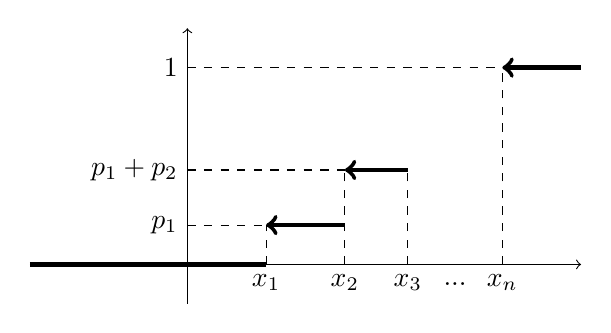
\begin{tikzpicture}[baseline={(current bounding box.center)}]
        \draw [->] (-2, 0) -- (5, 0);
        \draw [->] (0, -0.5) -- (0, 3);
        \draw [ultra thick] (-2, 0) -- (1, 0);
        \draw [dashed] (1, 0) -- (1, 0.5);
        \draw [ultra thick] [<-] (1, 0.5) -- (2, 0.5);
        \draw [dashed] (2, 0) -- (2, 1.2);
        \draw [ultra thick] [<-] (2, 1.2) -- (2.8, 1.2);
        \draw [dashed] (2.8, 0) -- (2.8, 1.2);
        \draw [dashed] (4, 0) -- (4, 2.5);
        \draw [ultra thick] [<-] (4, 2.5) -- (5, 2.5);
        \draw [dashed] (0, 2.5) -- (4, 2.5);
        \draw [dashed] (0, 0.5) -- (1, 0.5);
        \draw [dashed] (0, 1.2) -- (2, 1.2);
        \node [below] at (1, 0) {$x_1$};
        \node [below] at (2, 0) {$x_2$};
        \node [below] at (2.8, 0) {$x_3$};
        \node [below] at (3.4, -0.1) {$...$};
        \node [below] at (4, 0) {$x_n$};
        \node [left] at (0, 0.5) {$p_1$};
        \node [left] at (0, 1.2) {$p_1 + p_2$};
        \node [left] at (0, 2.5) {$1$};
    \end{tikzpicture} &
    $F_\xi(x) = \begin{cases}
        0, & x \leq x_1 \\
        p_1, & x_1 < x \leq x_2 \\
        p_1 + p_2, & x_2 < x \leq x_3 \\
        \dots \\
        \sum\limits_{i=1}^{n-1} p_i, & x_{n-1} < x \leq x_n \\
        \sum\limits_{i=1}^{n} p_i = 1, & x > x_n
    \end{cases}$
\end{tabular}